\documentclass[border=15pt]{standalone}
\usepackage{tikz,amsmath,amssymb}
\usetikzlibrary{arrows.meta,calc,shapes.geometric}
\usepackage{graphicx}
\usepackage{tikzcats}

% ========== 配色方案（参考 Inception 调色板） ==========
\definecolor{inFill}{RGB}{183,224,177}
\definecolor{inLine}{RGB}{32,102,32}
\definecolor{backFill}{RGB}{218,232,252}
\definecolor{backLine}{RGB}{55,95,170}
\definecolor{hidFill}{RGB}{199,203,243}
\definecolor{hidLine}{RGB}{52,58,143}
\definecolor{orFill}{RGB}{250,224,180}
\definecolor{orLine}{RGB}{190,110,20}
\definecolor{outFill}{RGB}{243,199,199}
\definecolor{outLine}{RGB}{143,52,52}
\definecolor{blFill}{RGB}{214,228,250}
\definecolor{blLine}{RGB}{60,90,170}
\definecolor{gapFill}{RGB}{236,220,248}
\definecolor{gapLine}{RGB}{125,50,150}
\definecolor{concatFill}{RGB}{252,242,185}
\definecolor{concatLine}{RGB}{180,145,20}
\definecolor{decFill}{RGB}{202,232,216}
\definecolor{decLine}{RGB}{28,110,75}
\definecolor{maskBg}{RGB}{35,40,52}
\definecolor{maskCat}{RGB}{230,60,50}

% 与 \cat 几何同构的语义分割掩码宏
\def\catmask#1{
\scope[scale=3]
    \draw[line width=15pt, #1, cap=round] (0,-2.3) .. controls +(-2,0) and (-2,-1.3) .. (-1.5,-1);
    \draw[line width=15pt, #1, cap=round] (-1.5,-1) .. controls +(0.9,0.4) and (-1.1,0.1) .. (-1.5,0);
    \fill[#1] (0.5,-2) circle (0.5);
    \fill[#1] (-0.5,-2) circle (0.5);
    \fill[#1, rounded corners=50pt] (-0.5,-2.5) rectangle (0.5,-0.3);
    \fill[#1] (0.4,-2.5) .. controls (0.3,-0.5) and (-0.3,-0.5) .. (-0.4,-2.5);
    \fill[#1] (0.4,-1.6) ellipse (0.2 and 0.9);
    \fill[#1, rounded corners=10pt] (0.6,-2.52) rectangle (0.2,-2.25);
    \fill[#1] (-0.4,-1.6) ellipse (0.2 and 0.9);
    \fill[#1, rounded corners=10pt] (-0.6,-2.52) rectangle (-0.2,-2.25);
    \fill[#1] (0,0) circle (0.65);
    \fill[rounded corners=8pt, #1] (0,0.5) -- (-0.6,1) -- (-0.7,0.8) -- (-0.6,0) -- cycle;
    \fill[rounded corners=8pt, #1] (0,0.5) -- (0.6,1) -- (0.7,0.8) -- (0.6,0) -- cycle;
    \fill[#1] (0,-0.5) ellipse (0.25 and 0.2);
    \draw[line width=1.5pt, #1, cap=round] (0.15,-0.34) .. controls (0.3,-0.31) and (0.6,-0.32) .. (0.8,-0.39);
    \draw[line width=1.5pt, #1, cap=round] (0.15,-0.39) .. controls (0.3,-0.36) and (0.55,-0.42) .. (0.75,-0.49);
    \draw[line width=1.5pt, #1, cap=round] (-0.15,-0.34) .. controls (-0.3,-0.31) and (-0.6,-0.32) .. (-0.8,-0.39);
    \draw[line width=1.5pt, #1, cap=round] (-0.15,-0.39) .. controls (-0.3,-0.36) and (-0.55,-0.42) .. (-0.75,-0.49);
\endscope
}

\begin{document}
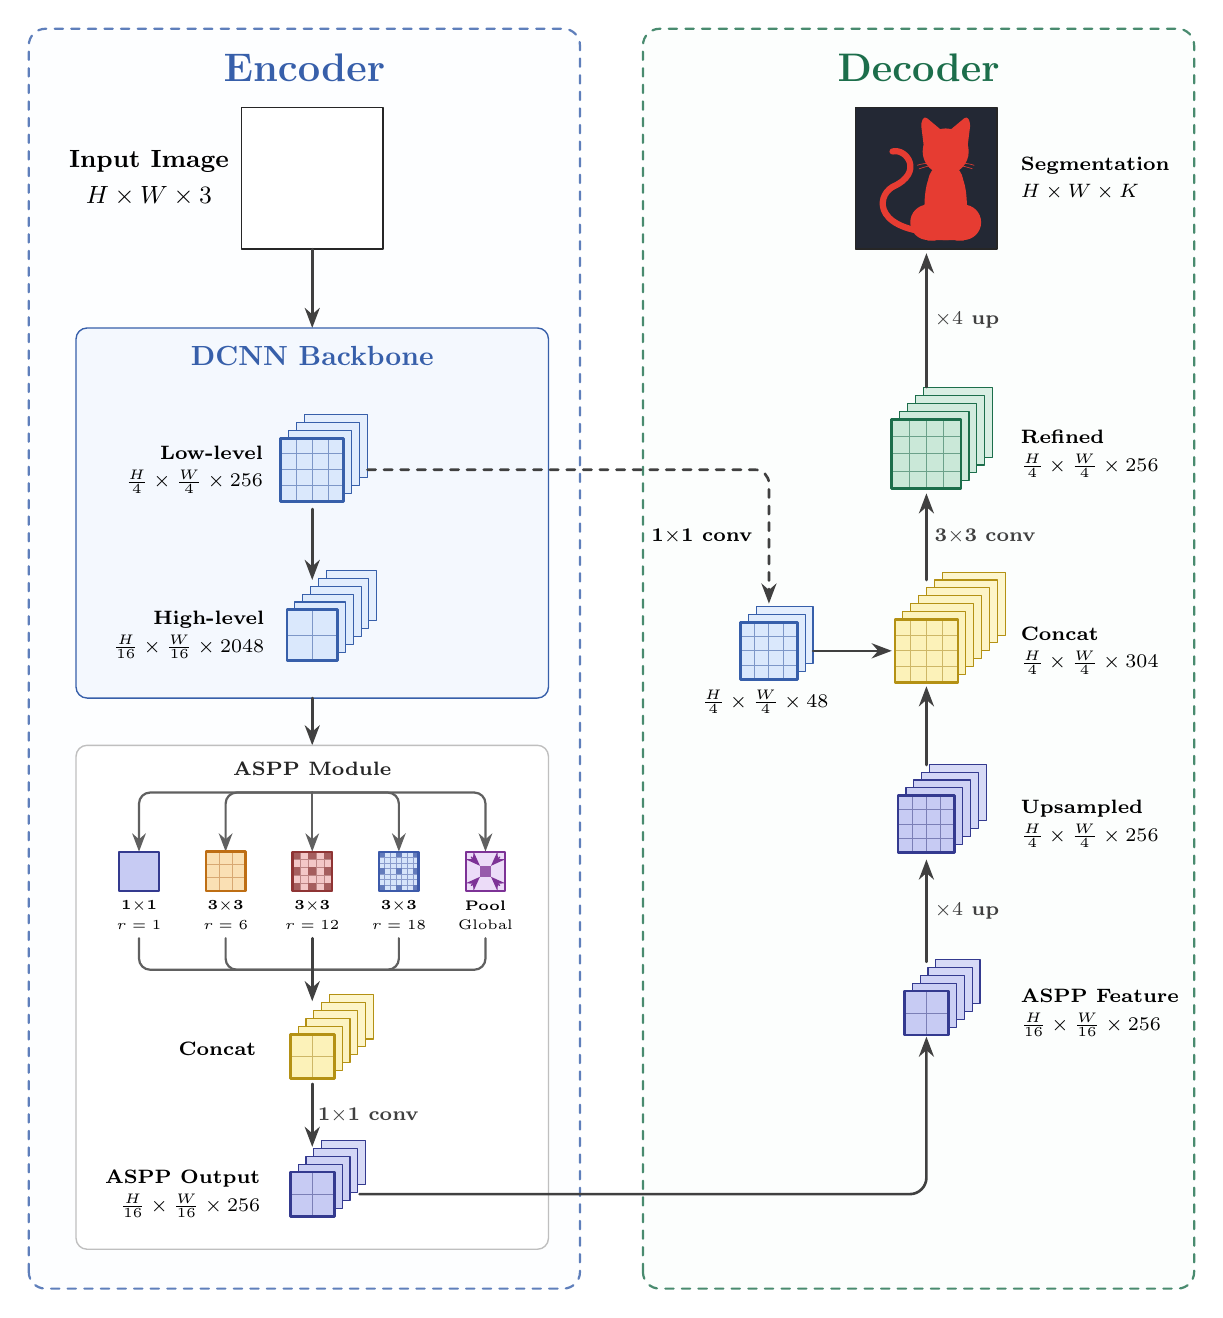
\begin{tikzpicture}[
    font=\small, line join=round, line cap=round,
    every node/.style={inner sep=0pt, outer sep=0pt, align=center},
    arr/.style={->, >=Stealth, line width=0.95pt, darkgray},
    skipArr/.style={->, >=Stealth, line width=0.95pt, darkgray, dashed},
    asppArr/.style={->, >=Stealth, line width=0.8pt, gray!75!black, rounded corners=4pt}
  ]

  % 宏：立体堆叠特征图
  \newcommand{\fstack}[6]{%
    \pgfmathsetmacro{\sz}{#4*#5}
    \pgfmathsetmacro{\half}{\sz/2}
    \foreach \k in {#3,...,1}{%
      \pgfmathtruncatemacro{\op}{round(100 - (28 * \k / #3))}
      \fill[#6Fill!\op, draw=#6Line, line width=.4pt]
        ({#1 - \half + 0.10*\k}, {#2 - \half + 0.10*\k}) rectangle ++({\sz}, {\sz});
    }
    \fill[#6Fill] ({#1 - \half}, {#2 - \half}) rectangle ++({\sz}, {\sz});
    \draw[step=#5, #6Line!65, line width=.35pt, shift={({#1 - \half}, {#2 - \half})}] (0,0) grid ({\sz}, {\sz});
    \draw[#6Line, line width=1.0pt] ({#1 - \half}, {#2 - \half}) rectangle ++({\sz}, {\sz});
  }

  % 宏：平面网格方块
  \newcommand{\gridbox}[5]{%
    \fill[#5Fill] (#1,#2) rectangle (#1+#3*#4, #2+#3*#4);
    \draw[step=#4, #5Line!60, line width=.3pt, shift={(#1,#2)}] (0,0) grid (#3*#4, #3*#4);
    \draw[#5Line, thick] (#1,#2) rectangle (#1+#3*#4, #2+#3*#4);
  }

  % 【左侧】：Encoder (保持不变，标题居中)
  \draw[draw=backLine!80, fill=backFill!6, dashed, line width=.8pt, rounded corners=6pt]
    (0.0, -3.8) rectangle (7.0, 12.2);
  \node[font=\Large\bfseries, text=backLine] at (3.5, 11.7) {Encoder};

  % 1. 顶部：输入原图
  \draw[black!85, line width=.6pt, fill=white] (2.7, 9.4) rectangle ++(1.8, 1.8);
  \node at (3.6, 10.3) {\scalebox{0.15}{\tikz{\cat}}};
  \node[right=6pt] at (0.3, 10.3) {\textbf{Input Image}\\[2pt]{$H \times W \times 3$}};

  \draw[arr] (3.6, 9.4) -- (3.6, 8.4);

  % 2. DCNN Backbone (宽 0.6 到 6.6，完全包住文字)
  \draw[draw=backLine, fill=backFill!30, rounded corners=4pt, line width=.5pt]
    (0.6, 3.7) rectangle (6.6, 8.4);
  \node[font=\bfseries, text=backLine] at (3.6, 8.05) {DCNN Backbone};

  % Low-level 特征
  \fstack{3.6}{6.6}{3}{4}{0.20}{back}
  \node[left=5pt, font=\scriptsize, align=right] at (3.15, 6.6) {
    \textbf{Low-level}\\[2pt]
    {$\frac{H}{4} \times \frac{W}{4} \times 256$}
  };

  \draw[arr] (3.6, 6.1) -- (3.6, 5.2);

  % Deep 特征 (High-level)
  \fstack{3.6}{4.5}{5}{2}{0.32}{back}
  \node[left=6pt, font=\scriptsize, align=right] at (3.2, 4.5) {
    \textbf{High-level}\\[2pt]
    {$\frac{H}{16} \times \frac{W}{16} \times 2048$}
  };

  \draw[arr] (3.6, 3.7) -- (3.6, 3.1);

  % 3. ASPP 模块 (外框与 Backbone 等宽 0.6 到 6.6)
  \draw[draw=gray!50, fill=white, rounded corners=4pt, line width=0.5pt]
    (0.6, -3.3) rectangle (6.6, 3.1);
  \node[font=\scriptsize\bfseries, text=black!85] at (3.6, 2.8) {ASPP Module};

  % ASPP 顶部分流：直接从 (3.6, 2.5) 到对应位置
  \draw[asppArr] (3.6, 2.5) -| (1.4, 1.75);
  \draw[asppArr] (3.6, 2.5) -| (2.5, 1.75);
  \draw[asppArr] (3.6, 2.5) -- (3.6, 1.75);
  \draw[asppArr] (3.6, 2.5) -| (4.7, 1.75);
  \draw[asppArr] (3.6, 2.5) -| (5.8, 1.75);

  % 分支 1: 1x1 conv (单框)
  \gridbox{1.15}{1.25}{1}{0.50}{hid}
  \node[below=2pt, font=\tiny] at (1.4, 1.2) {\textbf{1$\times$1}\\[1pt]{$r=1$}};

  % 分支 2: 3x3 conv (纯浅色网格)
  \gridbox{2.25}{1.25}{3}{0.167}{or}
  \node[below=2pt, font=\tiny] at (2.5, 1.2) {\textbf{3$\times$3}\\[1pt]{$r=6$}};

  % 分支 3: 3x3 空洞卷积 (rate=12)
  \begin{scope}[shift={(3.35, 1.25)}]
    \fill[outFill] (0,0) rectangle (0.5, 0.5);
    \draw[step=0.10, outLine!60, line width=.25pt] (0,0) grid (0.5, 0.5);
    \foreach \r in {0,2,4} \foreach \c in {0,2,4} {
      \fill[outLine!80] (\c*0.10, \r*0.10) rectangle ++(0.10, 0.10);
    }
    \draw[outLine, thick] (0,0) rectangle (0.5, 0.5);
  \end{scope}
  \node[below=2pt, font=\tiny] at (3.6, 1.2) {\textbf{3$\times$3}\\[1pt]{$r=12$}};

  % 分支 4: 3x3 空洞卷积 (rate=18)
  \begin{scope}[shift={(4.45, 1.25)}]
    \fill[blFill] (0,0) rectangle (0.5, 0.5);
    \draw[step=0.0714, blLine!60, line width=.25pt] (0,0) grid (0.5, 0.5);
    \foreach \r in {0,3,6} \foreach \c in {0,3,6} {
      \fill[blLine!80] (\c*0.0714, \r*0.0714) rectangle ++(0.0714, 0.0714);
    }
    \draw[blLine, thick] (0,0) rectangle (0.5, 0.5);
  \end{scope}
  \node[below=2pt, font=\tiny] at (4.7, 1.2) {\textbf{3$\times$3}\\[1pt]{$r=18$}};

  % 分支 5: Image Pooling
  \begin{scope}[shift={(5.55, 1.25)}]
    \fill[gapFill] (0,0) rectangle (0.5, 0.5);
    \draw[gapLine, thick] (0,0) rectangle (0.5, 0.5);
    \draw[->, >=Stealth, gapLine, line width=0.5pt] (0.07, 0.43) -- (0.18, 0.32);
    \draw[->, >=Stealth, gapLine, line width=0.5pt] (0.43, 0.43) -- (0.32, 0.32);
    \draw[->, >=Stealth, gapLine, line width=0.5pt] (0.07, 0.07) -- (0.18, 0.18);
    \draw[->, >=Stealth, gapLine, line width=0.5pt] (0.43, 0.07) -- (0.32, 0.18);
    \fill[gapLine!80] (0.18, 0.18) rectangle ++(0.14, 0.14);
  \end{scope}
  \node[below=2pt, font=\tiny] at (5.8, 1.2) {\textbf{Pool}\\[1pt]{Global}};

  % ASPP 底部分支合并
  \draw[line width=.8pt, gray!75!black, rounded corners=4pt] (1.4, 0.65) |- (3.6, 0.25);
  \draw[line width=.8pt, gray!75!black, rounded corners=4pt] (2.5, 0.65) |- (3.6, 0.25);
  \draw[line width=.8pt, gray!75!black, rounded corners=4pt] (4.7, 0.65) |- (3.6, 0.25);
  \draw[line width=.8pt, gray!75!black, rounded corners=4pt] (5.8, 0.65) |- (3.6, 0.25);
  \draw[arr] (3.6, 0.65) -- (3.6, -0.15);

  % ASPP Concat 特征
  \fstack{3.6}{-0.85}{5}{2}{0.28}{concat}
  \node[font=\scriptsize\bfseries, left=6pt] at (3.1, -0.75) {Concat};

  % 1x1 conv 降维
  \draw[arr] (3.6, -1.2) -- (3.6, -2.0)
    node[midway, right=2pt, font=\scriptsize\bfseries] {1$\times$1 conv};

  % ASPP 输出特征
  \fstack{3.6}{-2.6}{4}{2}{0.28}{hid}
  \node[left=6pt, font=\scriptsize, align=right] at (3.15, -2.6) {
    \textbf{ASPP Output}\\[2pt]
    {$\frac{H}{16} \times \frac{W}{16} \times 256$}
  };

  % 【右侧】：Decoder (优化对齐版，主轴 X = 11.4，侧边支路 X = 9.4)
  \draw[draw=decLine!80, fill=decFill!6, dashed, line width=.8pt, rounded corners=6pt]
    (7.8, -3.8) rectangle (14.8, 12.2);
  \node[font=\Large\bfseries, text=decLine] at (11.3, 11.7) {Decoder};

  % 底部单笔圆角连线：从 Encoder 输出横穿汇入主轴起点 (X = 11.4)
  \draw[arr, rounded corners=6pt] (4.2, -2.6) -- (11.4, -2.6) -- (11.4, -0.6);

  % 主轴层级 1: ASPP 特征
  \fstack{11.4}{-0.3}{4}{2}{0.28}{hid}
  \node[anchor=west, font=\scriptsize, align=left] at (12.6, -0.3) {
    \textbf{ASPP Feature}\\[2pt]
    {$\frac{H}{16} \times \frac{W}{16} \times 256$}
  };

  % 向上 x4 上采样
  \draw[arr] (11.4, 0.35) -- (11.4, 1.65)
    node[midway, right=3pt, font=\scriptsize\bfseries] {$\times 4$ up};

  % 主轴层级 2: 上采样特征
  \fstack{11.4}{2.1}{4}{4}{0.18}{hid}
  \node[anchor=west, font=\scriptsize, align=left] at (12.6, 2.1) {
    \textbf{Upsampled}\\[2pt]
    {$\frac{H}{4} \times \frac{W}{4} \times 256$}
  };

  % 向上送入 Concat
  \draw[arr] (11.4, 2.85) -- (11.4, 3.85);

  % 【侧边支路】：置于 X = 9.4，线条与文字完全隔开，下方仅保留尺寸
  \draw[skipArr, rounded corners=5pt] (4.3, 6.6) -- (9.4, 6.6) -- (9.4, 4.9);
  \node[left=6pt, font=\scriptsize\bfseries] at (9.4, 5.75) {1$\times$1 conv};

  % 1x1 降维后特征图 (中心 Y = 4.3 与 Concat 水平对齐)
  \fstack{9.4}{4.3}{2}{4}{0.18}{back}

  % 正下方直接标注尺寸公式
  \node[below=4pt, font=\scriptsize, align=center] at (9.4, 3.94) {
    {$\frac{H}{4} \times \frac{W}{4} \times 48$}
  };

  % 侧边特征图水平直插主轴 Concat
  \draw[arr] (9.96, 4.3) -- (10.96, 4.3);

  % 主轴垂直继续向上 (X = 11.4)
  % 主轴层级 3: Concat 特征图
  \fstack{11.4}{4.3}{6}{4}{0.20}{concat}
  \node[anchor=west, font=\scriptsize, align=left] at (12.6, 4.3) {
    \textbf{Concat}\\[2pt]
    {$\frac{H}{4} \times \frac{W}{4} \times 304$}
  };

  % 向上 3x3 conv 细化
  \draw[arr] (11.4, 5.2) -- (11.4, 6.3)
    node[midway, right=3pt, font=\scriptsize\bfseries] {3$\times$3 conv};

  % 主轴层级 4: 细化特征
  \fstack{11.4}{6.8}{4}{4}{0.22}{dec}
  \node[anchor=west, font=\scriptsize, align=left] at (12.6, 6.8) {
    \textbf{Refined}\\[2pt]
    {$\frac{H}{4} \times \frac{W}{4} \times 256$}
  };

  % 向上 x4 上采样
  \draw[arr] (11.4, 7.65) -- (11.4, 9.35)
    node[midway, right=3pt, font=\scriptsize\bfseries] {$\times 4$ up};

  % 主轴层级 5: 顶部输出分割图 (与左侧输入原图高度 10.3 严格齐平)
  \fill[maskBg] (10.5, 9.4) rectangle ++(1.8, 1.8);
  \draw[black!85, line width=.6pt] (10.5, 9.4) rectangle ++(1.8, 1.8);
  \node at (11.4, 10.3) {\scalebox{0.15}{\tikz{\catmask{maskCat}}}};
  \node[anchor=west, font=\scriptsize, align=left] at (12.6, 10.3) {
    \textbf{Segmentation}\\[2pt]
    {$H \times W \times K$}
  };
\end{tikzpicture}
\end{document}